\documentclass{article}
\usepackage[utf8]{inputenc}
\usepackage[T1]{fontenc}
\usepackage{polski}
\usepackage{indentfirst}
\usepackage{lastpage}
\usepackage{graphicx} 

\usepackage{fancyhdr}
\pagestyle{fancy}
\fancyhf{}
\rhead{Franciszek Wysocki, Bartosz Zdybel}
\rfoot{Strona \thepage \hspace{1pt} z \pageref{LastPage}}
\lhead{Spis treści}
\title{Specyfikacja funkcjonalna gry w czołgi \\ pt. „BattleZone”}
\author{}
\date{}

\begin{document}
\maketitle

\begin{flushright}
\par ...
\vfill
\par
Wykonali: Franciszek Wysocki, Bartosz Zdybel

Sprawdzający: mgr inż. Paweł Zawadzki

Data: 14.04.2020
\end{flushright}

\thispagestyle{empty}
\newpage
\begin{frame}{}
    \tableofcontents
\end{frame}
\newpage

\section{Cel dokumentu}
{\fontsize{14}{14}\selectfont
Niniejszy dokument przeznaczony jest dla końcowego użytkownika aplikacji. Jego celem jest opisanie w jaki sposób będzie można korzystać z programu - jakie bedą jego funkcje i ograniczenia. Ponadto dokument precyzuje jakie dane wejściowe będą niezbędne do uruchomienia, jakie dane wyjściowe zostaną wygenerowane oraz jak zostaną obsłużone sytuacje wyjątkowe.
}
\lhead{Cel i opis teoretyczny projektu}
\section{Cel i opis teoretyczny projektu}
{\fontsize{14}{14}\selectfont
Celem projektu jest stworzenie prostej gry/aplikacji z interfejsem graficznym wykorzystując język Java. Program będzie miał za zadanie wczytywać dane z pliku konfiguracyjnego, a następnie na ich podstawie uruchamiać grę. Podczas niej dwóch graczy będzie rywalizować o zdobycie jak największej liczby punktów poprzez zestrzeliwanie komórek. Gra skończy się wtedy gdy upłynie określony czas, któryś z graczy osiągnie maksymalną liczbe punktów przewidzianą na daną rozgrywkę lub specjalna komórka armagedon zostanie zniszczona. Końcowy stan gry będzie zapisywany do pliku graficznego.
}
\lhead{Założenia}
\section{Założenia}
{\fontsize{14}{14}\selectfont 


Rozgrywka będzie odbywać się na następujących zasadach, gracze będą:
\begin{itemize}

\item znajdować się po przeciwnych stronach planszy.
\item reprezentowani przez obiekty graficzne „czołgi”.
\item mogli poruszać lufą „czołgu” w zakresie $+/-45^{\circ} $.
\item mogli wystrzelić maksymalnie P pocisków.
\item mogli poruszać się wzdłuż pionowch krawędzi planszy.
\end{itemize}
\newpage
Pozostałe założenia gry niezależące od gracza:
\begin{itemize}
\item Każda komórka ma określoną wartość punktową, jaką zdobywa gracz, który jako ostatni odda strzał w daną komórkę.
\item Każda trafiona komórka dekrementuje swoją wartość o jeden.
\item Za uśmiercenie komórki gracz zdobywa taką ilość punktów jaką maksymalnie miała dana komórka.
\item Pod losowymi komórkami mogą wystąpić dodatkowe punkty - ,,punkty spadkowe''.
\item Punkty spadkowe mogą występować w wariantach: 10, 20, 30, 50, 100.
\item Każda komórka ma na sobie wyświetloną aktualną wartość oraz każda komórka ma kolor odpowiadający najwyższej wartości jaką dotychczas posiadała.
\item Na planszy znajduje się komórka armagedon (nie wyróżnia się ona wyglądem od innych komórek), a po jej zestrzeleniu zostaje zakończona gra.
\item W trakcie gry co Z sekund zwiększa się prędkość pocisków o K procent, a wielkość komórek zmniejsza się o Z procent.
\item Maksymalna prędkość pocisków może wynosić 300 procent początkowej, a komórka nie może zmaleć poniżej 50 procent.
\item Co kreślony czas rodzą się tzw. ,,komórki dzieci'' z wartością 1.
\end{itemize}

Dodatkowo w grze zostanie wyświetlona hierarchia kolorów komórek (poniżej pola bitwy) w celu łatwej oceny sytuacji przez gracza.


\newpage
}
\lhead{Uruchomienie programu}
\section{Uruchomienie programu}
{\fontsize{14}{14}\selectfont 
Program będzie uruchamiany z wiersza poleceń. Użytkownik będzie mógł podać nazwę pliku konfiguracyjnego jako argument wywołania. Plik ten musi posiadać rozszerzenie txt. Gdy użytkownik nie poda nazwy pliku zostanie wczytany domyślny plik konfiguracyjny z najbardziej optymalnymi ustawieniami. Użytkownik będzie miał możliwość również wprowadzania imion/nicków graczy, które wyświetlą się po stronie danego gracza.
}

\lhead{Przykładowy scenariusz uruchomienia}
\section{Przykładowy scenariusz uruchomienia}
{\fontsize{14}{14}\selectfont 
Scenariusz prawidłowego uruchomienia programu:
\begin{enumerate}
\item Użytkownik stworzy plik tekstowy z poprawnymi danymi wejściowymi o rozszerzeniu txt.
\item Użytkownik uruchomi program z nazwą powyższego pliku.
\item Program wygeneruje odpowiednią planszę i ustawi liczniki czasu według podanych parametrów.
\item Użytkownicy będą rywalizować między sobą o zdobycie jak największej liczby punktów poprzez oddawanie strzałów w komórki za pomocą przypisanych im klawiszy.
\item W przypadku którejkolwiek z trzech możliwości zakończenia rozgrywki nastąpi koniec gry oraz zostaną wypisane informacje o zwycięzcy rozgrywki.
\item Program stworzy obrazek png, w którym zapisze końcowy stan planszy.
\item Program zakończy działanie.
\end{enumerate}
}
\newpage
\lhead{Dane wejściowe}
\section{Dane wejściowe}
{\fontsize{14}{14}\selectfont 
Użytkownik przy uruchomieniu może podać plik tekstowy, musi przy tym wymienić w nim wszystkie parametry:
\begin{itemize}
\item wysokość i szerokość planszy,
\item P - ilość wystrzelonych pocisków,
\item H - czas po jakim pojawiają się komórki w losowych miejscach,
\item X - czas po jakim rodzą sie tzw. komórki dzieci, 
\item Y - czas po którym komórki żywe wzmacniają swoją siłę,
\item Z - czas po którym predkość pocisków się zmiększa,
\item K - procentowo o ile się zwiększa się predkość pocisków,
\item L - procentowo o ile zmniejsza się wielkośc komórek,
\item M - maksymalna ilość punktów przewidzainych na dana rozgrywkę,
\end{itemize}

\begin{figure}[h]
\centering
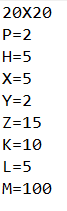
\includegraphics[width=2cm]{dane.png}
\caption{}
\label{fig:obrazek }
\end{figure}
}
Przykładowy plik wejściowy wygląda w sposób nastepujący (Rysunek 1):
\newpage
\lhead{Dane wyjściowe}
\section{Dane wyjściowe}
{\fontsize{14}{14}\selectfont 
Program zapisuje stan gry do pliku graficznego o rozszerzeniu png. Na obrazku będzie znajdować ostatnie ułożenie komórek na planszy wraz z uwzględnieniem ich wartościi kolorów.
}
\lhead{Komunikaty o błędach}
\section{Komunikaty o błędach}
{\fontsize{14}{14}\selectfont 
Komunikaty o błędach będą pojawiać się w wierszu poleceń w poniższych sytuacjach:
\begin{itemize}
\item Podanie pliku wejściowego z nieprawidłowym rozszerzeniem. Wymagane będzie txt.
\item Podanie błędnych danych w pliku.
\item Niepodanie wszystkich wymaganych stałych.
\item Podanie nazwy pliku, który nie istnieje.
\item Podanie nieodpowiedniej liczby argumentów.

\end{itemize}
}



\lhead{Sterowanie}
\section{Sterowanie}
{\fontsize{14}{14}\selectfont 
Sterowanie grą odbywać się będzie wyłącznie za pomocą klawiatury, a każdy z graczy będzie miał przypisane przyciski.


Gracz po lewej stronie będzie sterował klawiszami:
\begin{itemize}
    \item W - ruch czołgu w górę.
    \item S - ruch czołgu w dół plaszny.
    \item D - ruch armaty w dół planszy.
    \item A - ruch armaty w górę planszy.
    \item Spacja - wystrzał
\end{itemize}


Natomiast gracz po prawej stronie:
\begin{itemize}
    \item strzałka w górę - ruch czołgu w górę.
    \item strzałka w dół - ruch czołgu w dół plaszny.
    \item strzałka w lewo - ruch armaty w dół planszy.
    \item strzałka w prawo - ruch armaty w górę planszy.
    \item Enter - wystrzał
\end{itemize}

}


\lhead{Testowanie}
\section{Testowanie}
{\fontsize{14}{14}\selectfont 
W projekcie zostaną stworzone testy jednostkowe. Będą one dotyczyć sprawdzania konktretnych fragmentów funkcjonalności, 
dzięki czemu będą dokładniej precyzowały ewentualne miejsca powodujące błędy. 
Ich nazwy będą zaczynać się od słowa Test, a same pliki będą znajdować się w katalogu tests.
Maven będzie je automatycznie uruchamiał przy każdym budowaniu projektu i odrazu przerywał całą procedurę w przypadku wykrycia błędu.Testy będą pisane na bieżąco podczas powstawania kodu.
}


\end{document} 